\chapter{实验一:梯度下降单机优化}

\section{实验内容与要点介绍}

\subsection{实验内容与要求}

\subsubsection{实验内容}
\begin{itemize}
    \item 了解优化器的作用与构建方式(以PyTorch为例)
    \item 构建一阶确定性、一阶随机性优化算法,实现GD、SGD、Adam优化算法
    \item 分析确定性优化算法与随机性优化算法实验结果
\end{itemize}

\subsubsection{实验要求}
\begin{itemize}
    \item 在MNIST数据集上完成图像分类任务
    \item 实现GD、SGD、ADAM三种基于梯度的优化方法, 写出三个优化器类
    \item 绘制三种优化方法下的loss函数变化图像,通过loss图像及其他实验结果,分析三种优化方法的特点
\end{itemize}

\subsection{PyTorch优化器}

\subsubsection{优化器是干什么用的}

下面展示了一段简单的网络训练过程的代码,我们通过这段代码来理解PyTorch中优化器所发挥的作用。

\begin{lstlisting}
def train_loop(dataloader, model, loss_fn, optimizer):
    size = len(dataloader.dataset)
    for batch, (X, y) in enumerate(dataloader):
        # Compute prediction and loss
        pred = model(X)
        loss = loss_fn(pred, y)
        
        # Backpropagation
        optimizer.zero_grad()
        loss.backward()
        optimizer.step()
\end{lstlisting}
    
在这段代码中\graylstinline{model}为神经网络模型,通过\graylstinline{model(X)}调用了\graylstinline{model}中的\graylstinline{forward}方法,即进行正向传播,获得神经网络输出(第5行)。然后通过损失函数\graylstinline{loss_fn}计算神经网络输出\graylstinline{pred}与数据真实值或标签\graylstinline{y}的差距得到损失值\graylstinline{loss}(第6行)。
得到损失值后,通过反向传播(第10行),网络\graylstinline{model}中的各个参数对应的梯度将会得到更新,得到各个参数的梯度后,优化器\graylstinline{optimizer}便可以根据既定的优化算法来更新参数(第11行)。需要注意的是,神经网络的梯度参数并不是储存最近一次反向传播(即调用\graylstinline{loss.backward()})的结果,而是会将反向传播得到的梯度与当前储存的值相加。因此,我们需要第9行\graylstinline{optimizer.zero_grad()}来将神经网络\graylstinline{model}中储存的梯度值置为0。

如果你是第一次看到类似代码,你可能还会疑惑上述代码中优化器\graylstinline{optimizer}和\graylstinline{model}似乎并没有建立联系,那为什么优化器能处理\graylstinline{model}中的参数呢?这是因为在这个函数之外,\graylstinline{model}中的参数\graylstinline{model.parameters()}早就被喂给\graylstinline{optimizer}了:
\begin{lstlisting}
    optimizer = torch.optim.SGD(model.parameters(), lr=learning_rate)
\end{lstlisting}

\subsubsection{如何在优化器中实现自己的算法}

从上面的例子中可以看到,除了构建函数外,一个最简单的优化器只需要实现\graylstinline{zero_grad}和\graylstinline{step}方法即可。此处需要注意的有这几点:
\begin{itemize}
    \item 当我们手动更改\graphicspath{model}中参数或梯度的值时候,需要将其从计算图中分离。即在\graylstinline{zero_grad}方法中,应包含\graylstinline{param.grad.detach_()}。
    \item 使用Adam算法时,由于还需要上一步优化得到的状态,因此可在初始化函数中构建一个字典用来储存状态。
\end{itemize}


\subsection{几种算法回顾}

梯度下降 Gradient Descent:
\begin{align} 
w_{t+1} = w_t - \eta \nabla f(w_t)
\end{align}
随机梯度下降 Stochastic gradient descent:
\begin{align} 
w_{t+1} = w_t - \eta \nabla f_i(w_t)
\end{align}
Adam:
\begin{align} % amsmath package
    m_{t+1} & = \beta_1 m_t + (1-\beta_1) \nabla f(w_t)   \\
    g_{t+1} & = \beta_2 g_t + (1-\beta_2) (\nabla f(w_t))^2
\end{align}


\section{使用VSCode与本地环境调试运行}

如果你已经完成了本地环境配置(\S\ref{sec:local-env}),那就可以打开VSCode进行下面的操作了:

\begin{enumerate}
    \item 安装Python插件,如图\ref{fig:task1-vscode-extension-install-python}所示。
        \begin{figure}[htbp]
            \centering
            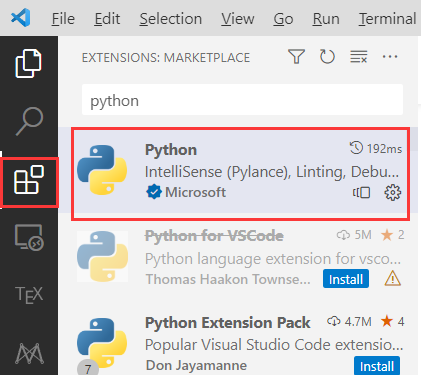
\includegraphics[width=0.7\textwidth]{figures/task1-vscode-extension-install-python.png}
            \caption{caption:task1-vscode-extension-install-python}
            \label{fig:task1-vscode-extension-install-python}
        \end{figure}
    \item 选择Python解释器,按下\graylstinline{F1}或\graylstinline{Ctrl + Shift + P},输入 "select interpreter"并选择 “Python: Select Interpreter”项(图\ref{fig:task1-vscode-local-select-interpreter})。然后选择:select at work space level。最后选择你在\S\ref{subsec:local-env-create}一孝节中创建的环境对应的解释器(图\ref{fig:task1-vscode-local-select-my-env}中为助教自己创建的distributedml环境)。
        \begin{figure}[htbp]
            \centering
            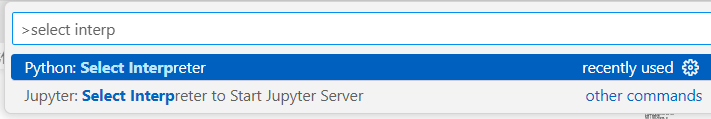
\includegraphics[width=0.7\textwidth]{figures/task1-vscode-local-select-interpreter.png}
            \caption{caption:task1-vscode-local-select-interpreter}
            \label{fig:task1-vscode-local-select-interpreter}
        \end{figure}
        \begin{figure}[htbp]
            \centering
            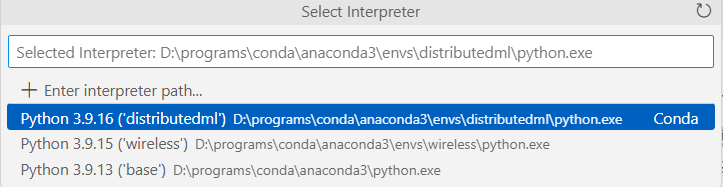
\includegraphics[width=0.7\textwidth]{figures/task1-vscode-local-select-my-env.png}
            \caption{caption:task1-vscode-local-select-my-env}
            \label{fig:task1-vscode-local-select-my-env}
        \end{figure}
    \item 最后,打开自己的.py文件,可以在编辑器右上角看到一个播放形状的三角,点击它或在下拉列表中选择运行或调试,即可开始运行或调试啦。
    \begin{figure}[htbp]
        \centering
        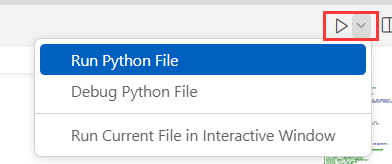
\includegraphics[width=0.5\textwidth]{figures/task1-vscode-local-run-or-debug.png}
        \caption{caption:task1-vscode-local-run-or-debug}
        \label{fig:task1-vscode-local-run-or-debug}
    \end{figure}
\end{enumerate}


\section{使用VSCode与本地容器调试运行}


\section{使用VSCode与远程服务器调试运行}

